\chapter{Espectroscopia electrónica y fotofísica}\label{ch:b3:electronic-spectroscopy}

Bajo la lámpara ultravioleta de un bar a oscuras, un vaso de tónica brilla con un
azul pálido, fantasmal. La quinina que contiene absorbe luz ultravioleta, que
el ojo no ve, y devuelve parte de ella unos nanosegundos después como
luz azul visible. Absorción, una vida breve en un estado excitado, emisión a
una longitud de onda mayor, la energía que no vuelve como luz: el destino de
una molécula excitada es una competición entre procesos con sus constantes de velocidad,
y su espectro está modelado por las vibraciones de la molécula y por las
reglas de simetría del \cref{ch:b3:group-theory-applied}. Este capítulo estudia
las transiciones electrónicas y lo que ocurre después de ellas, el campo llamado
fotofísica; el \cref{ch:b3:photochemistry} añade los casos en que la molécula
excitada reacciona.

\begin{recall}
El volumen del primer año midió la absorbancia con la ley de Beer--Lambert, $A =
\varepsilon\ell c$, definió el coeficiente de absorción molar, los cromóforos y
los sistemas conjugados, y relacionó el color con el máximo de absorción. El volumen del
segundo año dio nombre a los orbitales frontera HOMO y LUMO. El \cref{ch:b3:many-electron-atoms}
definió los \omterm{def:b3:many-electron-atoms:singlet-triplet}{estados singlete} y triplete; el \cref{ch:b3:group-theory-applied}, el
teorema de las integrales nulas; el \cref{ch:b3:rovibrational-spectroscopy}, los
niveles de vibración de un enlace.
\end{recall}

\begin{omfigure}
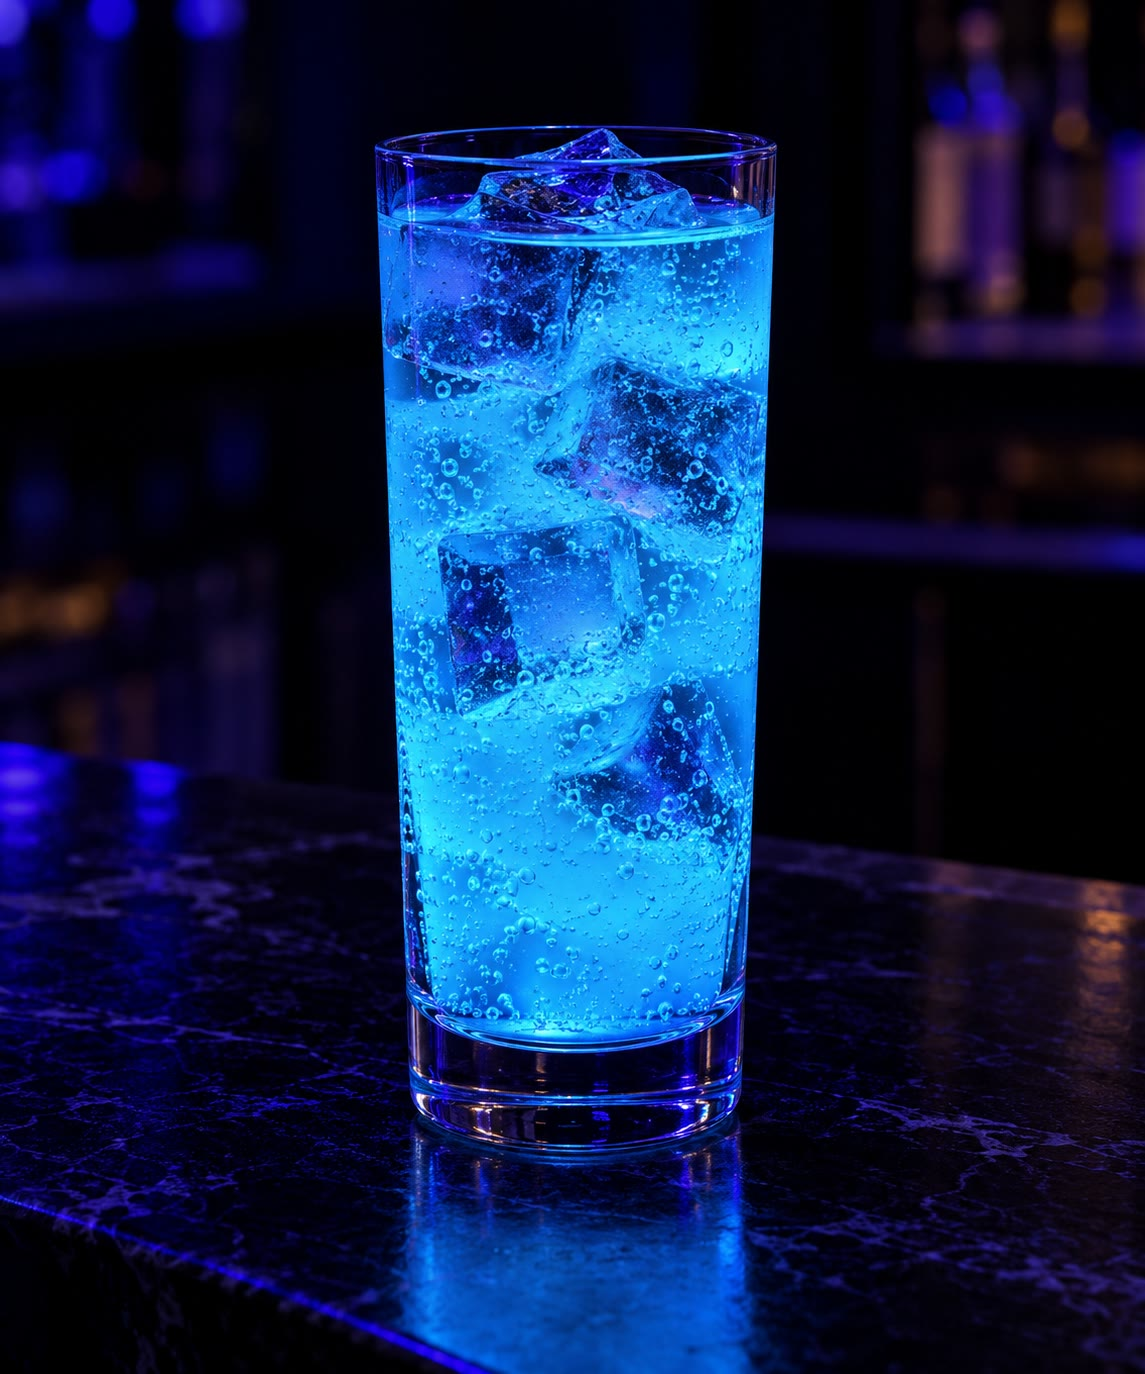
\includegraphics[height=4.6cm]{images/book4/ai/b3-07-tonic.jpg}\hspace{1em}%
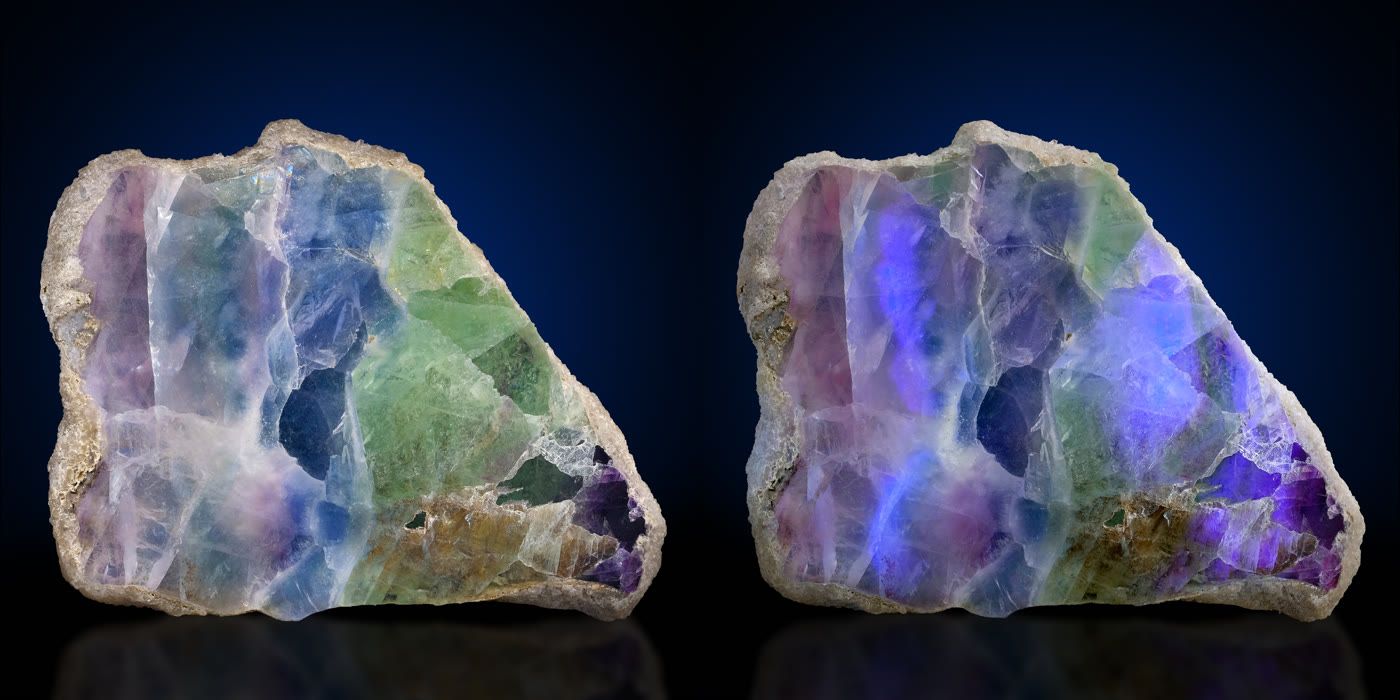
\includegraphics[height=4.6cm]{images/book4/fluorite-uv.jpg}

{\small Izquierda: agua tónica que brilla en azul bajo una lámpara ultravioleta. Derecha:
fluorita a la luz del día y emitiendo \omterm{def:b3:electronic-spectroscopy:luminescence}{fluorescencia} bajo luz ultravioleta; el mineral
dio nombre a la \omterm{def:b3:electronic-spectroscopy:luminescence}{fluorescencia}. Fotografía de Masha Milshina, CC BY 4.0.}
\end{omfigure}

\section{Las transiciones electrónicas y sus reglas de selección}

\begin{definition}[Momento dipolar de transición, fuerza del oscilador]\label{def:b3:electronic-spectroscopy:transition-dipole}
El \emph{momento dipolar de transición}\index{momento dipolar de transicion@momento dipolar de transición} entre
los estados $\Psi_i$ y $\Psi_f$ es $\boldsymbol\mu_{fi} = \langle\Psi_f|\hat{\boldsymbol\mu}|\Psi_i
\rangle$, con $\hat{\boldsymbol\mu} = -e\sum_k\mathbf r_k$ (más las cargas
nucleares, que se cancelan entre estados ortogonales). La \emph{fuerza del
oscilador}\index{fuerza del oscilador} $f$ es la medida adimensional de la
intensidad de una banda, del orden de 1 para las transiciones más intensas.
\end{definition}

\begin{proposition}[Intensidad y fuerza del oscilador]\label{prop:b3:electronic-spectroscopy:intensity}
La absorción integrada de una banda es proporcional a $|\boldsymbol\mu_{fi}|^2$,
y en la práctica
\[
f \approx 4.32\times10^{-9}\int\varepsilon(\tilde\nu)\,\dd\tilde\nu,
\]
con $\varepsilon$ en \unit{L.mol^{-1}.cm^{-1}} y $\tilde\nu$ en \unit{cm^{-1}}.
\end{proposition}
\admitted

La proporcionalidad procede de la teoría de perturbaciones dependiente del tiempo, y el
factor numérico, del oscilador clásico; ambos corresponden a cursos más
avanzados. Lo que importa aquí es que $f$ solo es grande cuando lo es
$\boldsymbol\mu_{fi}$, y que la simetría puede anularlo.

\begin{theorem}[La regla de selección de espín]\label{thm:b3:electronic-spectroscopy:spin-rule}
Una transición dipolar eléctrica entre estados de espín total distinto está
prohibida: $\Delta S = 0$.
\end{theorem}

\begin{proof}
Cada estado es el producto de una función espacial por una función de espín, $\Psi = \phi\,\chi$.
El \omterm{def:b3:quantum-model-systems:operator}{operador} dipolar solo actúa sobre las posiciones, luego $\langle\phi_f\chi_f|\hat{\boldsymbol\mu}|
\phi_i\chi_i\rangle = \langle\phi_f|\hat{\boldsymbol\mu}|\phi_i\rangle\langle\chi_f|\chi_i\rangle$.
Las funciones de espín de distinto $S$ son \omterm{def:b3:quantum-model-systems:operator}{funciones propias} de $\hat S^2$ con \omterm{def:b3:quantum-model-systems:operator}{valores propios}
distintos, y por tanto ortogonales (\cref{thm:b3:quantum-model-systems:hermitian-real}):
el segundo factor se anula.
\end{proof}

\begin{theorem}[La regla de Laporte]\label{thm:b3:electronic-spectroscopy:laporte}
En una molécula con \omterm{def:b3:point-groups:inversion}{centro de inversión}, una transición dipolar eléctrica debe
cambiar de paridad: $g \leftrightarrow u$ está permitida, $g \leftrightarrow g$ y $u
\leftrightarrow u$ están prohibidas. Es la \emph{regla de Laporte}\index{regla de Laporte}.
\end{theorem}

\begin{proof}
Las componentes de $\hat{\boldsymbol\mu}$ cambian de signo con la inversión: son $u$.
El producto $\Gamma_f\otimes\Gamma_\mu\otimes\Gamma_i$ solo es $g$ si $\Gamma_f$ y $\Gamma_i$
tienen paridades opuestas; en otro caso es $u$ y no puede contener la \omterm{def:b3:group-theory-applied:reducible}{representación
totalmente simétrica} (\cref{thm:b3:group-theory-applied:vanishing-integral}).
\end{proof}

Las dos reglas son estrictas para los estados idealizados; las moléculas reales las relajan
---el \omterm{def:b3:many-electron-atoms:spin-orbit}{acoplamiento espín--órbita} mezcla carácter singlete y triplete, las vibraciones
eliminan por un instante el centro de simetría--- y las transiciones ``prohibidas''
aparecen, débiles. Las bandas $d$--$d$ de los complejos octaédricos, prohibidas por la \omterm{thm:b3:electronic-spectroscopy:laporte}{regla de
Laporte} y débiles, deben su color a esta relajación
(\cref{ch:b3:complex-spectra-magnetism}).

\begin{definition}[Transición de transferencia de carga]\label{def:b3:electronic-spectroscopy:charge-transfer}
Una \emph{transición de transferencia de carga}\index{transicion de transferencia de carga@transición de transferencia de carga} lleva un
electrón de un orbital situado principalmente en una parte de un sistema (un dador) a
un orbital situado principalmente en otra (un aceptor); su dipolo de transición es
grande, su banda intensa y ancha, y su energía sensible a la polaridad del
disolvente.
\end{definition}

\begin{method}[Asignar una banda de absorción]\label{met:b3:electronic-spectroscopy:assign-band}
\begin{enumerate}
  \item $\varepsilon_{\max}$ por encima de unos \qty{e4}{L.mol^{-1}.cm^{-1}}: una transición
        permitida ($\pi\to\pi^*$ de un sistema conjugado, o de transferencia de carga).
  \item $\varepsilon_{\max}$ de 10 a unos cientos: una transición prohibida ($n\to\pi^*$,
        prohibida por simetría; $d$--$d$, prohibida por la \omterm{thm:b3:electronic-spectroscopy:laporte}{regla de Laporte}).
  \item $\varepsilon_{\max}$ inferior a 1: prohibida por el espín.
  \item Una banda $n\to\pi^*$ se desplaza hacia longitudes de onda más cortas en disolventes próticos
        (el par no enlazante se estabiliza por enlaces de hidrógeno), y una banda $\pi\to\pi^*$
        suele hacerlo hacia longitudes más largas.
\end{enumerate}
\end{method}

\section{El principio de Franck--Condon}

\begin{theorem}[Principio de Franck--Condon]\label{thm:b3:electronic-spectroscopy:franck-condon}
Dentro de la \omterm{def:b3:computational-chemistry:born-oppenheimer}{aproximación de Born--Oppenheimer}, y si el dipolo de transición
depende poco de las posiciones nucleares, la intensidad de la \omterm{def:b3:electronic-spectroscopy:vibronic}{transición
vibrónica} desde el nivel de vibración $v''$ del estado electrónico inferior hasta el nivel
$v'$ del superior es proporcional a $|\langle\chi_{v'}|\chi_{v''}\rangle|^2$, el
cuadrado del solapamiento de las dos funciones de onda de vibración: es el
\emph{principio de Franck--Condon}\index{principio de Franck--Condon}. Las transiciones
electrónicas son verticales: los núcleos no se mueven mientras los electrones saltan.
\end{theorem}

\begin{proof}
Con $\Psi = \psi_{\mathrm{el}}(\mathbf r;R)\chi_v(R)$, el momento de transición es
$\int\chi_{v'}^*\big[\int\psi'^*_{\mathrm{el}}\hat\mu\psi''_{\mathrm{el}}\dd\mathbf r\big]
\chi_{v''}\,\dd R$. El corchete es el momento de transición electrónico
$\mu_{\mathrm{el}}(R)$; tomado como constante (la aproximación de Condon), sale de
la integral y deja $\mu_{\mathrm{el}}\langle\chi_{v'}|\chi_{v''}\rangle$.
\end{proof}

\begin{definition}[Transición vibrónica, progresión, factor de Franck--Condon]\label{def:b3:electronic-spectroscopy:vibronic}
Una \emph{transición vibrónica}\index{transicion vibronica@transición vibrónica} cambia a la vez los estados
electrónico y de vibración; las rayas $v' \leftarrow 0$ para $v' = 0, 1, 2,
\dots$ forman una \emph{progresión vibrónica}\index{progresion vibronica@progresión vibrónica}; el
\emph{factor de Franck--Condon}\index{factor de Franck--Condon} de una raya vibrónica es
$|\langle\chi_{v'}|\chi_{v''}\rangle|^2$.
\end{definition}

\begin{proposition}[Osciladores desplazados]\label{prop:b3:electronic-spectroscopy:displaced}
Si ambos estados son armónicos con la misma frecuencia y el mínimo superior está
desplazado en $\Delta$ (en unidades de $\sqrt{\hbar/m\omega}$), los \omterm{def:b3:electronic-spectroscopy:vibronic}{factores de Franck--Condon}
desde $v'' = 0$ forman una distribución de Poisson,
$|\langle v'|0\rangle|^2 = \eu^{-S}S^{v'}/v'!$, con $S = \Delta^2/2$; la raya más intensa
está cerca de $v' = S$.
\end{proposition}
\admitted

La demostración general usa los \omterm{def:b3:quantum-model-systems:ladder}{operadores escalera} del
\cref{ch:b3:quantum-model-systems}; los datos de las figuras de este capítulo comprueban la
fórmula frente a la integración directa. Un desplazamiento pequeño da una sola raya 0--0
intensa; uno grande, una larga progresión cuyo miembro más intenso está lejos de
la raya 0--0.

\begin{omfigure}
\begin{tikzpicture}
\begin{axis}[name=pc, width=0.46\linewidth, height=6cm, xmin=-4, xmax=5, ymin=0,
  ymax=14, axis lines=left, xtick=\empty, ytick=\empty, xlabel={coordenada nuclear},
  ylabel={energía}, label style={font=\small}]
\addplot[black, thick] table[x=y, y=ground] {figdata/out/bachelor-3-franck-condon-curves.dat};
\addplot[omDef, thick] table[x=y, y=excited] {figdata/out/bachelor-3-franck-condon-curves.dat};
\draw[omabs] (axis cs:0,0.5) -- (axis cs:0,10.6);
\draw[omvib] (axis cs:-1,0.5) -- (axis cs:1,0.5);
\draw[omvib] (axis cs:0.732,9.5) -- (axis cs:2.732,9.5);
\draw[omvib] (axis cs:-0.000,10.5) -- (axis cs:3.464,10.5);
\draw[omvib] (axis cs:-0.504,11.5) -- (axis cs:3.968,11.5);
\draw[omvib] (axis cs:-0.914,12.5) -- (axis cs:4.378,12.5);
\node[font=\small, anchor=west] at (axis cs:-3.9,13.0) {excitado};
\node[font=\small, anchor=west] at (axis cs:3.0,1.5) {básico};
\node[font=\scriptsize, anchor=east] at (axis cs:-0.05,5.5) {vertical};
\end{axis}
\begin{axis}[at={(pc.east)}, anchor=west, xshift=1.3cm, width=0.46\linewidth,
  height=6cm, xmin=-0.5, xmax=12.5, ymin=0, ymax=0.8, axis lines=left, ycomb,
  xlabel={$v'$}, ylabel={factor de Franck--Condon}, label style={font=\small},
  tick label style={font=\small}]
\addplot[black, very thick] table[x=v, y=s03] {figdata/out/bachelor-3-franck-condon-sticks.dat};
\addplot[omDef, very thick, xshift=2pt] table[x=v, y=s15] {figdata/out/bachelor-3-franck-condon-sticks.dat};
\addplot[omThm, very thick, xshift=4pt] table[x=v, y=s5] {figdata/out/bachelor-3-franck-condon-sticks.dat};
\end{axis}
\end{tikzpicture}

{\small Izquierda: una transición vertical desde el nivel más bajo del estado fundamental
llega allí donde la curva excitada, desplazada hacia longitudes de enlace mayores, está muy por encima de
su mínimo (dibujada para $S = 1.5$). Derecha: \omterm{def:b3:electronic-spectroscopy:vibronic}{factores de Franck--Condon} de la
progresión para $S = 0.3$ (negro), 1.5 (azul) y 5 (rojo); cada conjunto suma
1.}
\end{omfigure}

\begin{example}[El yodo]\label{ex:b3:electronic-spectroscopy:iodine}
% ledger: diat:I2.re, diat:I2B.re, diat:I2B.we, imass:I127
El vapor de yodo es violeta porque su banda B$\leftarrow$X absorbe la luz amarillo-verdosa.
El enlace se alarga de \qty{266.6}{pm} en el estado fundamental a \qty{302.5}{pm} en
el estado B. En el modelo de osciladores desplazados con la frecuencia del estado B
(\qty{125.7}{cm^{-1}}), $\Delta R = \qty{35.8}{pm}$ da $S \approx 15$: la absorción es una
larga progresión cuyas rayas más intensas terminan en niveles de vibración altos del
estado B, y cuya continuación se adentra en el continuo de disociación.
\end{example}

\section{Los destinos de un estado excitado: el diagrama de Jablonski}

\begin{definition}[Diagrama de Jablonski]\label{def:b3:electronic-spectroscopy:jablonski}
Un \emph{diagrama de Jablonski}\index{diagrama de Jablonski} representa los estados electrónicos
de una molécula (singletes $S_0, S_1, S_2, \dots$ en una columna, tripletes $T_1, T_2,
\dots$ en otra), sus niveles de vibración y los procesos que los conectan:
los radiativos como flechas rectas, los no radiativos como flechas onduladas.
\end{definition}

\begin{definition}[Procesos no radiativos]\label{def:b3:electronic-spectroscopy:radiationless}
La \emph{relajación vibracional}\index{relajacion vibracional@relajación vibracional} lleva una molécula
excitada al nivel de vibración más bajo de su estado electrónico mediante
colisiones, en picosegundos. La \emph{conversión interna}\index{conversion interna@conversión interna}
es una transición no radiativa entre estados de la misma
multiplicidad ($S_2 \to S_1$, $S_1 \to S_0$); el \emph{cruce entre
sistemas}\index{cruce entre sistemas}, una transición entre estados de distinta
multiplicidad ($S_1 \to T_1$, $T_1 \to S_0$).
\end{definition}

\begin{definition}[Luminiscencia, fluorescencia, fosforescencia, desplazamiento de Stokes]\label{def:b3:electronic-spectroscopy:luminescence}
La \emph{luminiscencia}\index{luminiscencia} es la emisión de luz por una molécula
excitada. La \emph{fluorescencia}\index{fluorescencia} es una emisión permitida por el espín,
normalmente $S_1 \to S_0$, rápida (nanosegundos); la \emph{fosforescencia}\index{fosforescencia}
es una emisión prohibida por el espín, normalmente $T_1 \to S_0$, lenta (de milisegundos a
segundos). El \emph{desplazamiento de Stokes}\index{desplazamiento de Stokes} es la diferencia,
en energía, entre los máximos de absorción y de emisión.
\end{definition}

\begin{omfigure}
\begin{tikzpicture}[font=\small, >=Stealth]
  \foreach \y/\l in {0/{$S_0$}, 3.4/{$S_1$}, 5.6/{$S_2$}}{
    \draw[omstate] (0,\y) -- (3.6,\y); \node[anchor=east] at (-0.1,\y) {\l};
    \foreach \d in {0.25,0.5,0.75}{\draw[omvib] (0,\y+\d) -- (3.6,\y+\d);}}
  \draw[omstate] (5.0,2.5) -- (7.6,2.5); \node[anchor=west] at (7.7,2.5) {$T_1$};
  \foreach \d in {0.25,0.5,0.75}{\draw[omvib] (5.0,2.5+\d) -- (7.6,2.5+\d);}
  \draw[omabs] (0.3,0) -- (0.3,4.15) node[pos=0.35, left, font=\scriptsize, align=right] {absorción};
  \draw[omabs] (0.7,0) -- (0.7,5.85);
  \draw[omnonrad] (1.05,5.85) -- (1.05,5.6);
  \draw[omnonrad] (1.05,5.6) -- (1.05,3.4) node[pos=0.5, right, font=\scriptsize] {CI};
  \draw[omnonrad] (0.45,4.15) -- (0.45,3.42);
  \draw[omfluo] (1.7,3.4) -- (1.7,0.5) node[pos=0.5, right, font=\scriptsize, align=left] {fluores-\\cencia};
  \draw[omnonrad] (3.2,3.4) -- (3.2,0.02) node[pos=0.5, right, font=\scriptsize] {CI};
  \draw[omisc] (3.6,3.4) -- (5.0,3.1) node[pos=0.5, above, font=\scriptsize] {CES};
  \draw[omnonrad] (5.3,3.1) -- (5.3,2.52);
  \draw[omphos] (6.0,2.5) -- (6.0,0.5) node[pos=0.5, right, font=\scriptsize, align=left] {fosfores-\\cencia};
  \draw[omisc] (5.6,2.5) -- (3.7,0.02) node[pos=0.45, above left, font=\scriptsize, inner sep=1pt] {CES};
  \draw[omvib, dashed] (3.6,0.5) -- (6.0,0.5);
  \draw[omvib, dashed] (3.6,0.0) -- (7.6,0.0);
\end{tikzpicture}

{\small Un \omterm{def:b3:electronic-spectroscopy:jablonski}{diagrama de Jablonski}. Flechas rectas: absorción (azul), \omterm{def:b3:electronic-spectroscopy:luminescence}{fluorescencia}
(rojo), \omterm{def:b3:electronic-spectroscopy:luminescence}{fosforescencia} (naranja); flechas onduladas: \omterm{def:b3:electronic-spectroscopy:radiationless}{relajación vibracional} y
\omterm{def:b3:electronic-spectroscopy:radiationless}{conversión interna} (CI); flechas onduladas discontinuas: \omterm{def:b3:electronic-spectroscopy:radiationless}{cruce entre sistemas} (CES).
La emisión parte del nivel de vibración más bajo de $S_1$ o de $T_1$ y puede terminar
en cualquier nivel de $S_0$.}
\end{omfigure}

\begin{proposition}[Regla de Kasha]\label{prop:b3:electronic-spectroscopy:kasha}
La \omterm{def:b3:electronic-spectroscopy:luminescence}{luminiscencia} se produce, con muy pocas excepciones, desde el estado excitado más bajo
de una multiplicidad dada ($S_1$ o $T_1$), sea cual sea el estado excitado al principio:
es la \emph{regla de Kasha}\index{regla de Kasha}.
\end{proposition}
\begin{proof}[Estatus]
Establecida experimentalmente; la razón es que la \omterm{def:b3:electronic-spectroscopy:radiationless}{conversión interna} entre los
estados excitados superiores, muy próximos entre sí, es mucho más rápida que la emisión,
mientras que la separación $S_1$--$S_0$ es grande.
\end{proof}

\begin{proposition}[Imagen especular]\label{prop:b3:electronic-spectroscopy:mirror}
Si los estados excitado y fundamental tienen una estructura de vibración parecida, la
banda de \omterm{def:b3:electronic-spectroscopy:luminescence}{fluorescencia} es la imagen especular de la primera banda de absorción respecto de su
raya 0--0 común; la emisión está a longitudes de onda mayores (\omterm{def:b3:electronic-spectroscopy:luminescence}{desplazamiento de Stokes}).
\end{proposition}

\begin{proof}
La absorción va de $v'' = 0$ a los niveles $v'$ de $S_1$, a $E_{00} + v'h\nu'$; la emisión,
de $v' = 0$ a los niveles $v''$ de $S_0$, a $E_{00} - v''h\nu''$. Con frecuencias
iguales y los mismos \omterm{def:b3:electronic-spectroscopy:vibronic}{factores de Franck--Condon} (igual desplazamiento), las dos
progresiones son simétricas respecto de $E_{00}$.
\end{proof}

\begin{omfigure}
\begin{tikzpicture}
\begin{axis}[width=0.75\linewidth, height=5cm, xmin=17, xmax=33, ymin=0,
  ymax=1.15, axis x line=bottom, axis y line=left, ytick=\empty,
  xlabel={número de onda / $10^3$ cm$^{-1}$}, ylabel={intensidad},
  legend cell align=left, legend style={font=\small, draw=none, at={(0.02,0.97)}, anchor=north west},
  tick label style={font=\small}, label style={font=\small}]
\addplot[omDef, thick] table[x=nu, y=abs] {figdata/out/bachelor-3-photophysics-bands.dat};
\addlegendentry{absorción}
\addplot[omThm, thick] table[x=nu, y=em] {figdata/out/bachelor-3-photophysics-bands.dat};
\addlegendentry{fluorescencia}
\draw[gray, dashed] (axis cs:25,0) -- (axis cs:25,1.12);
\node[font=\scriptsize, gray, anchor=south west] at (axis cs:25,1.0) {0--0};
\end{axis}
\end{tikzpicture}

{\small Absorción y \omterm{def:b3:electronic-spectroscopy:luminescence}{fluorescencia} de una molécula modelo ($S = 1$, cuanto de
vibración de \qty{1400}{cm^{-1}}): imágenes especulares respecto de la raya 0--0; los máximos están
separados por el \omterm{def:b3:electronic-spectroscopy:luminescence}{desplazamiento de Stokes}.}
\end{omfigure}

\section{Cinética de los estados excitados}

Tras la excitación, la población de $S_1$ decae por todos los procesos que tiene a su alcance,
cada uno de primer orden: desexcitación radiativa $k_r$, \omterm{def:b3:electronic-spectroscopy:radiationless}{conversión interna} $k_{\mathrm{IC}}$,
\omterm{def:b3:electronic-spectroscopy:radiationless}{cruce entre sistemas} $k_{\mathrm{ISC}}$.

\begin{definition}[Tiempo de vida del estado excitado, tiempo de vida radiativo]\label{def:b3:electronic-spectroscopy:lifetime}
El \emph{tiempo de vida del estado excitado}\index{tiempo de vida del estado excitado} es $\tau =
1/\sum k$, la constante de tiempo del decaimiento exponencial de la población
excitada. El \emph{tiempo de vida radiativo}\index{tiempo de vida radiativo} $\tau_r =
1/k_r$ es el tiempo de vida que tendría el estado si la emisión fuera su único
destino.
\end{definition}

\begin{definition}[Rendimiento cuántico]\label{def:b3:electronic-spectroscopy:quantum-yield}
El \emph{rendimiento cuántico}\index{rendimiento cuantico@rendimiento cuántico} de un proceso que sigue a la
absorción de luz es el número de sucesos de ese proceso dividido por el
número de fotones absorbidos. El \emph{rendimiento cuántico de
fluorescencia}\index{rendimiento cuantico de fluorescencia@rendimiento cuántico de fluorescencia} $\Phi_F$ es el número de fotones
emitidos como \omterm{def:b3:electronic-spectroscopy:luminescence}{fluorescencia} por fotón absorbido.
\end{definition}

\begin{proposition}[Rendimiento cuántico y tiempo de vida]\label{prop:b3:electronic-spectroscopy:quantum-yield}
$\Phi_F = k_r/(k_r + k_{\mathrm{IC}} + k_{\mathrm{ISC}}) = k_r\tau = \tau/\tau_r$; del mismo modo,
$\Phi_{\mathrm{ISC}} = k_{\mathrm{ISC}}\tau$, y los rendimientos de los procesos en competencia
suman 1.
\end{proposition}

\begin{proof}
$\dd[S_1]/\dd t = -(k_r + k_{\mathrm{IC}} + k_{\mathrm{ISC}})[S_1]$, luego $[S_1] = [S_1]_0\eu^{-t/\tau}$.
El número de fotones emitidos es $\int_0^\infty k_r[S_1]\,\dd t = k_r\tau[S_1]_0$, de
$[S_1]_0$ moléculas excitadas. La misma integral con cada $k$ da cada rendimiento,
y su suma es $\tau\sum k = 1$.
\end{proof}

\begin{definition}[Extintor de fluorescencia, extinción dinámica y estática]\label{def:b3:electronic-spectroscopy:quencher}
Un \emph{extintor de fluorescencia}\index{extintor de fluorescencia} es una especie que
reduce la \omterm{def:b3:electronic-spectroscopy:luminescence}{fluorescencia}. En la \emph{extinción dinámica}\index{extincion dinamica@extinción dinámica}
desactiva la molécula excitada al chocar con ella, lo que añade una velocidad $k_q[Q]$ y
acorta el tiempo de vida; en la \emph{extinción estática}\index{extincion estatica@extinción estática}
forma un complejo no fluorescente con la molécula en estado fundamental, lo que reduce la
intensidad sin cambiar el tiempo de vida de las moléculas que siguen emitiendo.
\end{definition}

\begin{theorem}[Ecuación de Stern--Volmer]\label{thm:b3:electronic-spectroscopy:stern-volmer}
Para la \omterm{def:b3:electronic-spectroscopy:quencher}{extinción dinámica},
\[
\frac{I_0}{I} = \frac{\tau_0}{\tau} = 1 + k_q\tau_0[Q] = 1 + K_{SV}[Q],
\]
es la \emph{ecuación de Stern--Volmer}\index{ecuacion de Stern--Volmer@ecuación de Stern--Volmer}, donde $I_0$ y $\tau_0$
se miden sin extintor y $K_{SV} = k_q\tau_0$.
\end{theorem}

\begin{proof}
Con extintor, $\tau = 1/(k_0 + k_q[Q])$ con $k_0 = 1/\tau_0$, luego $\tau_0/\tau = 1 +
k_q\tau_0[Q]$. La intensidad es proporcional a $\Phi_F = k_r\tau$, luego $I_0/I = \tau_0/\tau$.
\end{proof}

\begin{omfigure}
\begin{tikzpicture}
\begin{axis}[name=dec, width=0.5\linewidth, height=5cm, xmin=0, xmax=40, ymode=log,
  ymin=0.005, ymax=1.2, axis lines=left, xlabel={$t$ / ns}, ylabel={$I(t)/I(0)$},
  legend cell align=left, legend style={font=\scriptsize, draw=none, at={(0.98,0.98)}, anchor=north east},
  tick label style={font=\small}, label style={font=\small}]
\addplot[black, thick] table[x=t, y=q0] {figdata/out/bachelor-3-photophysics-decays.dat};
\addlegendentry{$[Q] = 0$}
\addplot[omDef, thick] table[x=t, y=q1] {figdata/out/bachelor-3-photophysics-decays.dat};
\addlegendentry{0.01 M}
\addplot[omProp, thick] table[x=t, y=q2] {figdata/out/bachelor-3-photophysics-decays.dat};
\addlegendentry{0.02 M}
\addplot[omThm, thick] table[x=t, y=q4] {figdata/out/bachelor-3-photophysics-decays.dat};
\addlegendentry{0.04 M}
\end{axis}
\begin{axis}[at={(dec.east)}, anchor=west, xshift=1.4cm, width=0.42\linewidth,
  height=5cm, xmin=0, xmax=0.045, ymin=0, ymax=3.3, axis lines=left,
  xlabel={$[Q]$ / mol L$^{-1}$}, ylabel={$I_0/I = \tau_0/\tau$},
  xticklabel style={/pgf/number format/fixed, /pgf/number format/precision=2},
  scaled x ticks=false, tick label style={font=\small}, label style={font=\small}]
\addplot[omThm, thick, mark=*] table[x=Q, y=I0I] {figdata/out/bachelor-3-photophysics-sv.dat};
\end{axis}
\end{tikzpicture}

{\small \omterm{def:b3:electronic-spectroscopy:quencher}{Extinción dinámica} de un fluoróforo modelo ($\tau_0 = \qty{10}{ns}$, $k_q =
\qty{5e9}{L.mol^{-1}.s^{-1}}$). Izquierda: decaimientos de \omterm{def:b3:electronic-spectroscopy:luminescence}{fluorescencia}, rectas en escala
logarítmica, más pronunciadas cuanto más extintor hay. Derecha: la recta de Stern--Volmer, de pendiente
$K_{SV} = k_q\tau_0 = \qty{50}{L/mol}$.}
\end{omfigure}

\begin{method}[Rendimiento cuántico de fluorescencia relativo]\label{met:b3:electronic-spectroscopy:relative-yield}
\begin{enumerate}
  \item Elegir un patrón de $\Phi_{\mathrm{std}}$ conocido que absorba a la misma
        longitud de onda de excitación.
  \item Preparar disoluciones diluidas ($A < 0.1$, para evitar la reabsorción) y registrar
        sus absorbancias $A$ y sus espectros de emisión integrados $F$ en condiciones
        idénticas.
  \item $\Phi = \Phi_{\mathrm{std}}\,\dfrac{F}{F_{\mathrm{std}}}\,\dfrac{A_{\mathrm{std}}}{A}\,
        \dfrac{n^2}{n_{\mathrm{std}}^2}$; el último factor corrige la diferencia de índices de
        refracción de los disolventes.
\end{enumerate}
\end{method}

\begin{method}[Analizar datos de extinción]\label{met:b3:electronic-spectroscopy:stern-volmer}
\begin{enumerate}
  \item Representar $I_0/I$ en función de $[Q]$; una recta que pasa por 1 da $K_{SV}$.
  \item Medir también los tiempos de vida: si $\tau_0/\tau$ sigue la misma recta, la extinción
        es dinámica y $k_q = K_{SV}/\tau_0$; si $\tau$ no cambia, es estática.
  \item Comparar $k_q$ con el límite de difusión, de unos \qty{e10}{L.mol^{-1}.s^{-1}} en
        agua (\cref{ch:b3:rate-theories}): un $k_q$ próximo a él significa que casi cada
        encuentro desactiva.
\end{enumerate}
\end{method}

\begin{example}[Quinina y antraceno]\label{ex:b3:electronic-spectroscopy:quinine}
% ledger: fl:quinine.labs, fl:quinine.eps, fl:quinine.phi, fl:anthracene.labs, fl:anthracene.phi
El sulfato de quinina en ácido sulfúrico \qty{0.5}{M} absorbe a \qty{349}{nm} con $\varepsilon =
\qty{5700}{L.mol^{-1}.cm^{-1}}$ y emite \omterm{def:b3:electronic-spectroscopy:luminescence}{fluorescencia} con $\Phi_F = 0.546$, lo que lo convierte en el
patrón clásico de los \omterm{def:b3:electronic-spectroscopy:quantum-yield}{rendimientos cuánticos} relativos. El antraceno en ciclohexano
absorbe a \qty{356}{nm} y tiene $\Phi_F = 0.36$; la mayor parte del resto de sus moléculas
excitadas pasa al triplete.
\end{example}

\section{Aplicaciones}

La \omterm{def:b3:electronic-spectroscopy:luminescence}{fluorescencia} se detecta sobre un fondo oscuro, lo que hace la fluorimetría
de cien a mil veces más sensible que la espectroscopia de absorción:
se miden de forma rutinaria concentraciones nanomolares de un compuesto fluorescente.
Las sondas fluorescentes informan de su entorno a través de su longitud de onda,
su rendimiento o su tiempo de vida (polaridad, pH, la fijación de un ion); la transferencia de energía
entre dos fluoróforos, eficaz solo a distancias de unos pocos nanómetros, mide
distancias en las proteínas. Los complejos fosforescentes de metales pesados, en los que el
\omterm{def:b3:many-electron-atoms:spin-orbit}{acoplamiento espín--órbita} hace eficaz el \omterm{def:b3:electronic-spectroscopy:radiationless}{cruce entre sistemas}, recogen los tripletes
en los diodos emisores de luz de las pantallas.

\begin{inthelab}[Recuento de fotones individuales correlacionado en el tiempo]
Para medir un tiempo de vida de nanosegundos, la muestra se excita con un diodo láser
pulsado a una frecuencia de repetición de megahercios y, para cada pulso, se registra el retraso del
primer fotón de \omterm{def:b3:electronic-spectroscopy:luminescence}{fluorescencia} detectado. Tras millones de pulsos, el
histograma de retrasos es la curva de decaimiento, a la que se ajusta $\tau$, con la
respuesta del instrumento medida sobre una disolución difusora. La fuente
ultravioleta está confinada; el operador trabaja con gafas que bloquean su
longitud de onda.
\end{inthelab}

\begin{history}[Stokes, 1852]
George Gabriel Stokes hizo pasar luz solar por un vidrio violeta y un prisma
hasta una disolución de quinina, y vio salir luz azul de la región iluminada por
rayos ultravioleta invisibles: la luz emitida tenía siempre una longitud de onda mayor
que la luz absorbida. Llamó al fenómeno \omterm{def:b3:electronic-spectroscopy:luminescence}{fluorescencia}, por el
mineral fluorita, que brilla de la misma manera.
\end{history}

\section{Ejercicios}

\begin{exercise}[$\star$]\label{exo:b3:electronic-spectroscopy:1}
¿Permitida o prohibida, y por qué regla?: (a) $S_0 \to T_1$ en el benceno; (b) una transición
$d$--$d$ de un complejo octaédrico; (c) la transición $\pi\to\pi^*$ del eteno
($B_{1u} \leftarrow A_g$ en $D_{2h}$); (d) la transición $n\to\pi^*$ del metanal
($A_2$).
\end{exercise}

\begin{exercise}[$\star$]\label{exo:b3:electronic-spectroscopy:2}
Un compuesto absorbe a \qty{349}{nm} y emite \omterm{def:b3:electronic-spectroscopy:luminescence}{fluorescencia} con un máximo a
\qty{450}{nm} (datos del ejercicio). Calcúlese el \omterm{def:b3:electronic-spectroscopy:luminescence}{desplazamiento de Stokes} en \unit{cm^{-1}} y en
eV.
\end{exercise}

\begin{exercise}[$\star$]\label{exo:b3:electronic-spectroscopy:3}
% ledger: fl:quinine.eps
Calcúlese la absorbancia a \qty{349}{nm} de una disolución de sulfato de quinina de \qty{1.0e-5}{mol/L}
en una cubeta de \qty{1}{cm}, y la fracción de la luz que absorbe.
\end{exercise}

\begin{exercise}[$\star$]\label{exo:b3:electronic-spectroscopy:4}
Un fluoróforo tiene $\Phi_F = 0.60$ y $\tau = \qty{4.0}{ns}$. Calcúlense $k_r$, el
\omterm{def:b3:electronic-spectroscopy:lifetime}{tiempo de vida radiativo} y la suma de las constantes de velocidad no radiativas.
\end{exercise}

\begin{exercise}[$\star\star$]\label{exo:b3:electronic-spectroscopy:5}
Una banda es gaussiana, con $\varepsilon_{\max} = \qty{5700}{L.mol^{-1}.cm^{-1}}$ y una anchura total a
media altura de \qty{5000}{cm^{-1}}. Estímese su \omterm{def:b3:electronic-spectroscopy:transition-dipole}{fuerza del oscilador} (la integral
de una gaussiana es $1.0645\,\varepsilon_{\max}\times$FWHM).
\end{exercise}

\begin{exercise}[$\star\star$]\label{exo:b3:electronic-spectroscopy:6}
Para osciladores desplazados, encuéntrese la raya más intensa de la progresión para
$S = 0.3$, 1.5 y 5, y la razón entre su factor y el de la raya 0--0.
\end{exercise}

\begin{exercise}[$\star\star$]\label{exo:b3:electronic-spectroscopy:7}
Desde $S_1$, $k_r = \qty{1.0e8}{s^{-1}}$, $k_{\mathrm{IC}} = \qty{2.0e7}{s^{-1}}$ y $k_{\mathrm{ISC}} =
\qty{3.0e8}{s^{-1}}$. Calcúlense $\tau$, $\Phi_F$ y $\Phi_{\mathrm{ISC}}$.
\end{exercise}

\begin{exercise}[$\star\star$]\label{exo:b3:electronic-spectroscopy:8}
% ledger: fl:quinine.phi, nD:water, nD:cyclohexane
La \omterm{def:b3:electronic-spectroscopy:luminescence}{fluorescencia} del antraceno en ciclohexano ($A = 0.040$) integra 0.46
veces la del sulfato de quinina en ácido sulfúrico diluido ($A = 0.050$, $\Phi =
0.546$). Con índices de refracción de 1.4266 (ciclohexano) y 1.333 (agua, para el
ácido diluido), calcúlese el $\Phi_F$ del antraceno.
\end{exercise}

\begin{exercise}[$\star\star$]\label{exo:b3:electronic-spectroscopy:9}
El tiempo de vida de un fluoróforo es 8.0, 5.6 y \qty{4.3}{ns} para concentraciones de
extintor de 0, 0.010 y \qty{0.020}{mol/L}. ¿Es dinámica la extinción? Encuéntrense
$K_{SV}$ y $k_q$.
\end{exercise}

\begin{exercise}[$\star\star\star$]\label{exo:b3:electronic-spectroscopy:10}
La adición de un extintor reduce a la mitad la intensidad de \omterm{def:b3:electronic-spectroscopy:luminescence}{fluorescencia}, mientras que el tiempo de vida
medido se mantiene en \qty{6.0}{ns}. ¿Qué tipo de extinción es, y qué implica
sobre el estado fundamental? Escríbase la relación correspondiente entre $I_0/I$
y la constante de asociación del complejo.
\end{exercise}

\begin{exercise}[$\star\star\star$]\label{exo:b3:electronic-spectroscopy:11}
% ledger: fl:anthracene.phi
El antraceno en ciclohexano tiene $\Phi_F = 0.36$ y, en las condiciones de una
medida, $\tau = \qty{5.0}{ns}$ (datos del ejercicio). Calcúlense $\tau_r$ y el
rendimiento del triplete si la \omterm{def:b3:electronic-spectroscopy:radiationless}{conversión interna} es despreciable. ¿Por qué es el
\omterm{def:b3:electronic-spectroscopy:lifetime}{tiempo de vida radiativo} más largo que el medido?
\end{exercise}

\begin{exercise}[$\star\star\star$]\label{exo:b3:electronic-spectroscopy:12}
Para dos electrones, la función de espín singlete es $\frac{1}{\sqrt2}[\alpha\beta - \beta\alpha]$
y la función triplete con $M_S = 0$ es $\frac{1}{\sqrt2}[\alpha\beta + \beta\alpha]$. Demuéstrese que
son ortogonales y conclúyase sobre la intensidad de $T_1 \leftarrow S_0$ en
ausencia de \omterm{def:b3:many-electron-atoms:spin-orbit}{acoplamiento espín--órbita}.
\end{exercise}

\section{Problema: por qué brilla el agua tónica}

\begin{problem}[{Problema de fin de semana --- la absorción de la quinina, el destino de su
estado excitado, la extinción por los iones cloruro y si cada encuentro
desactiva}]
\label{pb:b3:electronic-spectroscopy:1}
% ledger: fl:quinine.labs, fl:quinine.eps, fl:quinine.phi, visc:H2O.25C
Sulfato de quinina en ácido sulfúrico \qty{0.5}{M}: máximo de absorción a \qty{349}{nm},
$\varepsilon = \qty{5700}{L.mol^{-1}.cm^{-1}}$, $\Phi_F = 0.546$. Datos del problema: el
tiempo de vida de \omterm{def:b3:electronic-spectroscopy:luminescence}{fluorescencia} sin extintor es $\tau_0 = \qty{19}{ns}$; el máximo de emisión
está cerca de \qty{450}{nm}; la adición de cloruro de sodio da las razones de intensidad
\begin{center}\small
\begin{tabular}{lccccc}
\hline
$[\ce{Cl-}]$ / mol L$^{-1}$ & 0 & 0.010 & 0.020 & 0.040 & 0.080 \\
$I_0/I$ & 1.000 & 1.594 & 2.188 & 3.376 & 5.752 \\ \hline
\end{tabular}
\end{center}
El agua a \qty{25}{\celsius} tiene una viscosidad de \qty{0.890}{mPa.s}; $R =
\qty{8.314}{J.K^{-1}.mol^{-1}}$.

\medskip\noindent\textbf{Parte I --- Absorción.}
\begin{enumerate}
  \item Calcúlese la absorbancia a \qty{349}{nm} de una disolución de \qty{1.0e-4}{mol/L} en una
        cubeta de \qty{1}{cm}.
  \item ¿Qué fracción de la luz incidente se absorbe?
  \item ¿Está permitida la transición? Úsese $\varepsilon$.
  \item Dese la energía del fotón absorbido en eV.
  \item ¿Por qué el ojo no ve ningún color de absorción en el agua tónica?
  \item ¿Por qué una disolución para trabajos de \omterm{def:b3:electronic-spectroscopy:luminescence}{fluorescencia} se mantiene por debajo de $A = 0.1$?
\end{enumerate}

\medskip\noindent\textbf{Parte II --- El estado excitado.}
\begin{enumerate}[resume]
  \item Dibújese el \omterm{def:b3:electronic-spectroscopy:jablonski}{diagrama de Jablonski} de los procesos que parten de $S_1$.
  \item Calcúlense la constante de velocidad radiativa $k_r$ y el \omterm{def:b3:electronic-spectroscopy:lifetime}{tiempo de vida radiativo}.
  \item Calcúlese la constante de velocidad no radiativa total.
  \item Calcúlese el \omterm{def:b3:electronic-spectroscopy:luminescence}{desplazamiento de Stokes} en \unit{cm^{-1}}.
  \item ¿Por qué la emisión es azul si la absorción está en el ultravioleta?
  \item ¿Qué fracción de la energía absorbida sale como \omterm{def:b3:electronic-spectroscopy:luminescence}{fluorescencia}, contando
        la energía de cada fotón?
\end{enumerate}

\medskip\noindent\textbf{Parte III --- La extinción por el cloruro.}
\begin{enumerate}[resume]
  \item Represéntese $I_0/I$ en función de $[\ce{Cl-}]$ y compruébese que es lineal.
  \item Determínese $K_{SV}$ por mínimos cuadrados con los cinco puntos.
  \item Suponiendo una \omterm{def:b3:electronic-spectroscopy:quencher}{extinción dinámica}, calcúlese $k_q$.
  \item ¿Qué tiempo de vida se mediría a \qty{0.040}{mol/L}?
  \item ¿Cómo se probaría experimentalmente que la extinción es dinámica?
  \item ¿Por qué el agua tónica, que no contiene cloruro, es un buen lugar para que
        brille la quinina?
\end{enumerate}

\medskip\noindent\textbf{Parte IV --- ¿Cada encuentro?}
\begin{enumerate}[resume]
  \item La constante de velocidad de los encuentros controlados por la difusión en un disolvente de
        viscosidad $\eta$ es $k_d \approx 8RT/3\eta$. Calcúlese en \unit{L.mol^{-1}.s^{-1}}.
  \item Compárense $k_q$ y $k_d$.
  \item ¿Qué fracción de los encuentros conduce a la extinción?
  \item ¿Sería la extinción más rápida o más lenta en un disolvente más viscoso?
  \item Enúnciese el resultado: la razón $k_q/k_d$ para la extinción de la quinina por el
        cloruro.
\end{enumerate}
\end{problem}
